
%%%%%%%%%%%%%%%%%%%%%%%%%%%%%%%%%%%%%%%%%%%%%%%%%%%%%%%%%%%%%%%%%%%%%%%%%%%%%%%%%%%%%%%
%%%%%%%%%%%%%%%%%%%%%%%%%%%%%%%%%%%%%%%%%%%%%%%%%%%%%%%%%%%%%%%%%%%%%%%%%%%%%%%%%%%%%%%
% 
% This top part of the document is called the 'preamble'.  Modify it with caution!
%
% The real document starts below where it says 'The main document starts here'.

\documentclass[12pt]{article}
\usepackage{hyperref}

\usepackage{amssymb,amsmath,amsthm}
\usepackage[top=1in, bottom=1in, left=1.25in, right=1.25in]{geometry}
\usepackage{fancyhdr}
\usepackage{enumerate}
\usepackage{listings}
\usepackage{graphicx}
\usepackage{float}
\usepackage{multicol}
% Comment the following line to use TeX's default font of Computer Modern.
\usepackage{times,txfonts}
\usepackage{mwe}
\usepackage{caption}
\usepackage{subcaption}

\usepackage{tikz}
\def\checkmark{\tikz\fill[scale=0.4](0,.35) -- (.25,0) -- (1,.7) -- (.25,.15) -- cycle;} 



\makeatletter
\renewcommand*\env@matrix[1][*\c@MaxMatrixCols c]{%
  \hskip -\arraycolsep
  \let\@ifnextchar\new@ifnextchar
  \array{#1}}
\makeatother

\newtheoremstyle{homework}% name of the style to be used
  {18pt}% measure of space to leave above the theorem. E.g.: 3pt
  {12pt}% measure of space to leave below the theorem. E.g.: 3pt
  {}% name of font to use in the body of the theorem
  {}% measure of space to indent
  {\bfseries}% name of head font
  {:}% punctuation between head and body
  {2ex}% space after theorem head; " " = normal interword space
  {}% Manually specify head
\theoremstyle{homework} 

% Set up an Exercise environment and a Solution label.
\newtheorem*{exercisecore}{\@currentlabel}
\newenvironment{exercise}[1]
{\def\@currentlabel{#1}\exercisecore}
{\endexercisecore}

\newcommand{\localhead}[1]{\par\smallskip\noindent\textbf{#1}\nobreak\\}%
\newcommand\solution{\localhead{Solution:}}

%%%%%%%%%%%%%%%%%%%%%%%%%%%%%%%%%%%%%%%%%%%%%%%%%%%%%%%%%%%%%%%%%%%%%%%%
%
% Stuff for getting the name/document date/title across the header
\makeatletter
\RequirePackage{fancyhdr}
\pagestyle{fancy}
\fancyfoot[C]{\ifnum \value{page} > 1\relax\thepage\fi}
\fancyhead[L]{\ifx\@doclabel\@empty\else\@doclabel\fi}
\fancyhead[C]{\ifx\@docdate\@empty\else\@docdate\fi}
\fancyhead[R]{\ifx\@docauthor\@empty\else\@docauthor\fi}
\headheight 15pt

\def\doclabel#1{\gdef\@doclabel{#1}}
\doclabel{Use {\tt\textbackslash doclabel\{MY LABEL\}}.}
\def\docdate#1{\gdef\@docdate{#1}}
\docdate{Use {\tt\textbackslash docdate\{MY DATE\}}.}
\def\docauthor#1{\gdef\@docauthor{#1}}
\docauthor{Use {\tt\textbackslash docauthor\{MY NAME\}}.}
\makeatother

% Shortcuts for blackboard bold number sets (reals, integers, etc.)
\newcommand{\Reals}{\ensuremath{\mathbb R}}
\newcommand{\Nats}{\ensuremath{\mathbb N}}
\newcommand{\Ints}{\ensuremath{\mathbb Z}}
\newcommand{\Rats}{\ensuremath{\mathbb Q}}
\newcommand{\Cplx}{\ensuremath{\mathbb C}}
%% Some equivalents that some people may prefer.
\let\RR\Reals
\let\NN\Nats
\let\II\Ints
\let\CC\Cplx

%\textbf{Code:}
%\begin{center}
%  \lstinputlisting{NewtonsMethodP5.m}
%\end{center}
%
%\textbf{Console:}
%\begin{center}
%  \lstinputlisting{P5C.txt}
%\end{center}
%\vspace{.15in}


%\begin{figure}[H]
%  \begin{center}
%    \caption{The one-norm unit ball}
%    \includegraphics[width=.76\textwidth]{1norm.png}
%  \end{center}
%\end{figure}




%%%%%%%%%%%%%%%%%%%%%%%%%%%%%%%%%%%%%%%%%%%%%%%%%%%%%%%%%%%%%%%%%%%%%%%%%%%%%%%%%%%%%%%
%%%%%%%%%%%%%%%%%%%%%%%%%%%%%%%%%%%%%%%%%%%%%%%%%%%%%%%%%%%%%%%%%%%%%%%%%%%%%%%%%%%%%%%
% 
% The main document start here.

% The following commands set up the material that appears in the header.
\doclabel{Math 615: Homework 7}
\docauthor{Stefano Fochesatto}
\docdate{\today}


\begin{document}


\begin{exercise}{Problem P30} Consider the "$\theta$-methods" for $u' = f(t, u)$, namely
  \begin{equation*}
    U^{n + 1} = U^n + k[(1 - \theta)f(t_n, U^n) + \theta f(t_{n + 1} U^{n+1})]
  \end{equation*}
  where $0 \leq \theta \leq 1$ is a fixed parameter. 
  \begin{enumerate}
    \item[\textbf{a.}] Cases $\theta = 0 ,1/2, 1$ are all familiar methods. Name them. 
    \solution 

    \begin{equation*}
      \theta = 0: \qquad U^{n + 1} = U^n + k[f(t_n, U^n)] \qquad \to \qquad \text{Forward Euler}
    \end{equation*}
    \begin{equation*}
      \theta = 1/2: \qquad  U^{n + 1} = U^n + \frac{k}{2}[f(t_n, U^n) + f(t_{n + 1} U^{n+1})] \qquad \to \qquad \text{Trapezoid Method}
    \end{equation*}
    \begin{equation*}
      \theta = 1: \qquad  U^{n + 1} = U^n + k[f(t_{n + 1} U^{n+1})] \qquad \to \qquad \text{Backward Euler}
    \end{equation*}




    \item[\textbf{b.}] Find the (absolute) stability regions for $\theta = 0, 1/4, 1/2, 3/4, 1$
    \solution Applying the test equation $u' = \lambda u$ to our general scheme we get, 
    \begin{equation*}
      U^{n + 1} = U^n + k[(1 - \theta)\lambda U^n + \theta \lambda U^{n+1}].
    \end{equation*}
    Solving for $U^{n+1} = R(z)U^n$ we get, 
    \begin{align*}
      U^{n + 1} &= U^n + k[(1 - \theta)\lambda U^n + \theta \lambda U^{n+1}]\\
      U^{n + 1} &= U^n + (1 - \theta)k\lambda U^n + \theta k\lambda U^{n+1}\\
      U^{n + 1} - \theta k\lambda U^{n+1} &= U^n + (1 - \theta)k\lambda U^n\\
      (1 - \theta k\lambda) U^{n+1} &= (1 + (1 - \theta)k\lambda) U^n\\
     U^{n+1} &= \dfrac{(1 + (1 - \theta)k\lambda)}{ (1 - \theta k\lambda) } U^n
    \end{align*}
    Plotting the stability region, for $\theta = 0$ first note that,
    \begin{equation*}
      R(z) = \dfrac{(1 + (1 - \theta)k\lambda)}{ (1 - \theta k\lambda) } = (1 + k\lambda) = 1 + z
    \end{equation*}
    Therefore the stability region is given by 
    \begin{align*}
      |1 + z| &\leq 1\\
      |1 + x + iy| &\leq 1\\
      (1 + x)^2 + y^2 &\leq 1\\
    \end{align*}
    \begin{figure}[H]
     \begin{center}
       \caption{Stability Region for $\theta = 0$ Method.}
       \includegraphics[width=.80\textwidth]{theta1.png}
     \end{center}
    \end{figure}









    Plotting the stability region, for $\theta = 1/4$ first note that,
    \begin{equation*}
      R(z) = \dfrac{(1 + \frac{3}{4}k\lambda)}{ (1 - \frac{1}{4} k\lambda) } = \dfrac{(1 + \frac{3}{4}z)}{ (1 - \frac{1}{4} z) }
    \end{equation*}
    Therefore the stability region is given by 
    \begin{align*}
      \left|\dfrac{(1 + \frac{3}{4}z)}{ (1 - \frac{1}{4} z) }\right| &\leq 1\\
      \left|\dfrac{(1 + \frac{3}{4}(x + iy))}{ (1 - \frac{1}{4}(x + iy)) }\right| &\leq 1\\
      \left|1 + \frac{3}{4}x + i\frac{3}{4}y\right| &\leq \left|1 - \frac{1}{4}x + i\frac{1}{4}y\right|\\
      (1 + \frac{3}{4}x)^2 + (\frac{3}{4}y)^2 &\leq (1 - \frac{1}{4}x)^2 + (\frac{1}{4}y)^2\\
      x^2 + 4x + y^2 &\leq 0\\
      (x^2 + 4x + 4) + y^2 &\leq 4\\
      (x + 2)^2 + y^2 &\leq 2^2
    \end{align*}

  \begin{figure}[H]
   \begin{center}
     \caption{Stability Region for $\theta = 1/4$ Method.}
     \includegraphics[width=.80\textwidth]{theta2.png}
   \end{center}
  \end{figure}



    Plotting the stability region, for $\theta = 1/2$ first note that,
    \begin{equation*}
      R(z) = \dfrac{(1 + \frac{1}{2}k\lambda)}{ (1 - \frac{1}{2} k\lambda) } = \dfrac{(1 + \frac{1}{2}z)}{ (1 - \frac{1}{2}z) }
    \end{equation*}
    Therefore the stability region is given by 
    \begin{align*}
      \left|\dfrac{(1 + \frac{1}{2}z)}{ (1 - \frac{1}{2} z) }\right| &\leq 1\\
      \left|\dfrac{(1 + \frac{1}{2}(x + iy))}{ (1 - \frac{1}{2}(x + iy)) }\right| &\leq 1\\
      \left|1 + \frac{1}{2}x + i\frac{1}{2}y\right| &\leq \left|1 - \frac{1}{2}x + i\frac{1}{2}y\right|\\
      (1 + \frac{1}{2}x)^2 + (\frac{1}{2}y)^2 &\leq (1 - \frac{1}{2}x)^2 + (\frac{1}{2}y)^2\\
      \frac{1}{4}x^2 + x + 1 + \frac{1}{4}y^2 &\leq \frac{1}{4}x^2 - x + 1 + \frac{1}{4}y^2\\
      x&\leq -x
    \end{align*}

    \begin{figure}[H]
      \begin{center}
        \caption{Stability Region for $\theta = 1/2$ Method.}
        \includegraphics[width=.80\textwidth]{theta3.png}
      \end{center}
     \end{figure}




    Plotting the stability region, for $\theta = 3/4$ first note that,
    \begin{equation*}
      R(z) = \dfrac{(1 + \frac{1}{4}k\lambda)}{ (1 - \frac{3}{4} k\lambda) } = \dfrac{(1 + \frac{1}{4}z)}{ (1 - \frac{3}{4} z) }
    \end{equation*}
    Therefore the stability region is given by 
    \begin{align*}
      \left|\dfrac{(1 + \frac{1}{4}z)}{ (1 - \frac{3}{4} z) }\right| &\leq 1\\
      \left|\dfrac{(1 + \frac{1}{4}(x + iy))}{ (1 - \frac{3}{4}(x + iy)) }\right| &\leq 1\\
      \left|1 + \frac{1}{4}x + i\frac{1}{4}y\right| &\leq \left|1 - \frac{3}{4}x + i\frac{3}{4}y\right|\\
      (1 + \frac{1}{4}x)^2 + (\frac{1}{4}y)^2 &\leq (1 - \frac{3}{4}x)^2 + (\frac{3}{4}y)^2\\
      y^2 - 4x + x^2 &\geq 0\\
      y^2 + 4 - 4x + x^2 &\geq 4\\
      y^2 + (x - 2)^2 &\geq 2^2
    \end{align*}

    \begin{figure}[H]
      \begin{center}
        \caption{Stability Region for $\theta = 3/4$ Method.}
        \includegraphics[width=.80\textwidth]{theta4.png}
      \end{center}
     \end{figure}


    Plotting the stability region, for $\theta = 1$ first note that,
    \begin{equation*}
      R(z) = \dfrac{(1 + (1 - \theta)k\lambda)}{ (1 - \theta k\lambda) } = \frac{1}{1 - k\lambda} = \frac{1}{1 - z} 
    \end{equation*}
    Therefore the stability region is given by,
    \begin{align*}
      \dfrac{1}{1 - z} &\leq 1\\
      \dfrac{1}{|1 - x - iy|} &\leq 1\\
      |1 - x - iy| &\geq 1\\
      (1 - x)^2 + y^2 &\geq 1
    \end{align*}

    \begin{figure}[H]
      \begin{center}
        \caption{Stability Region for $\theta = 1$ Method.}
        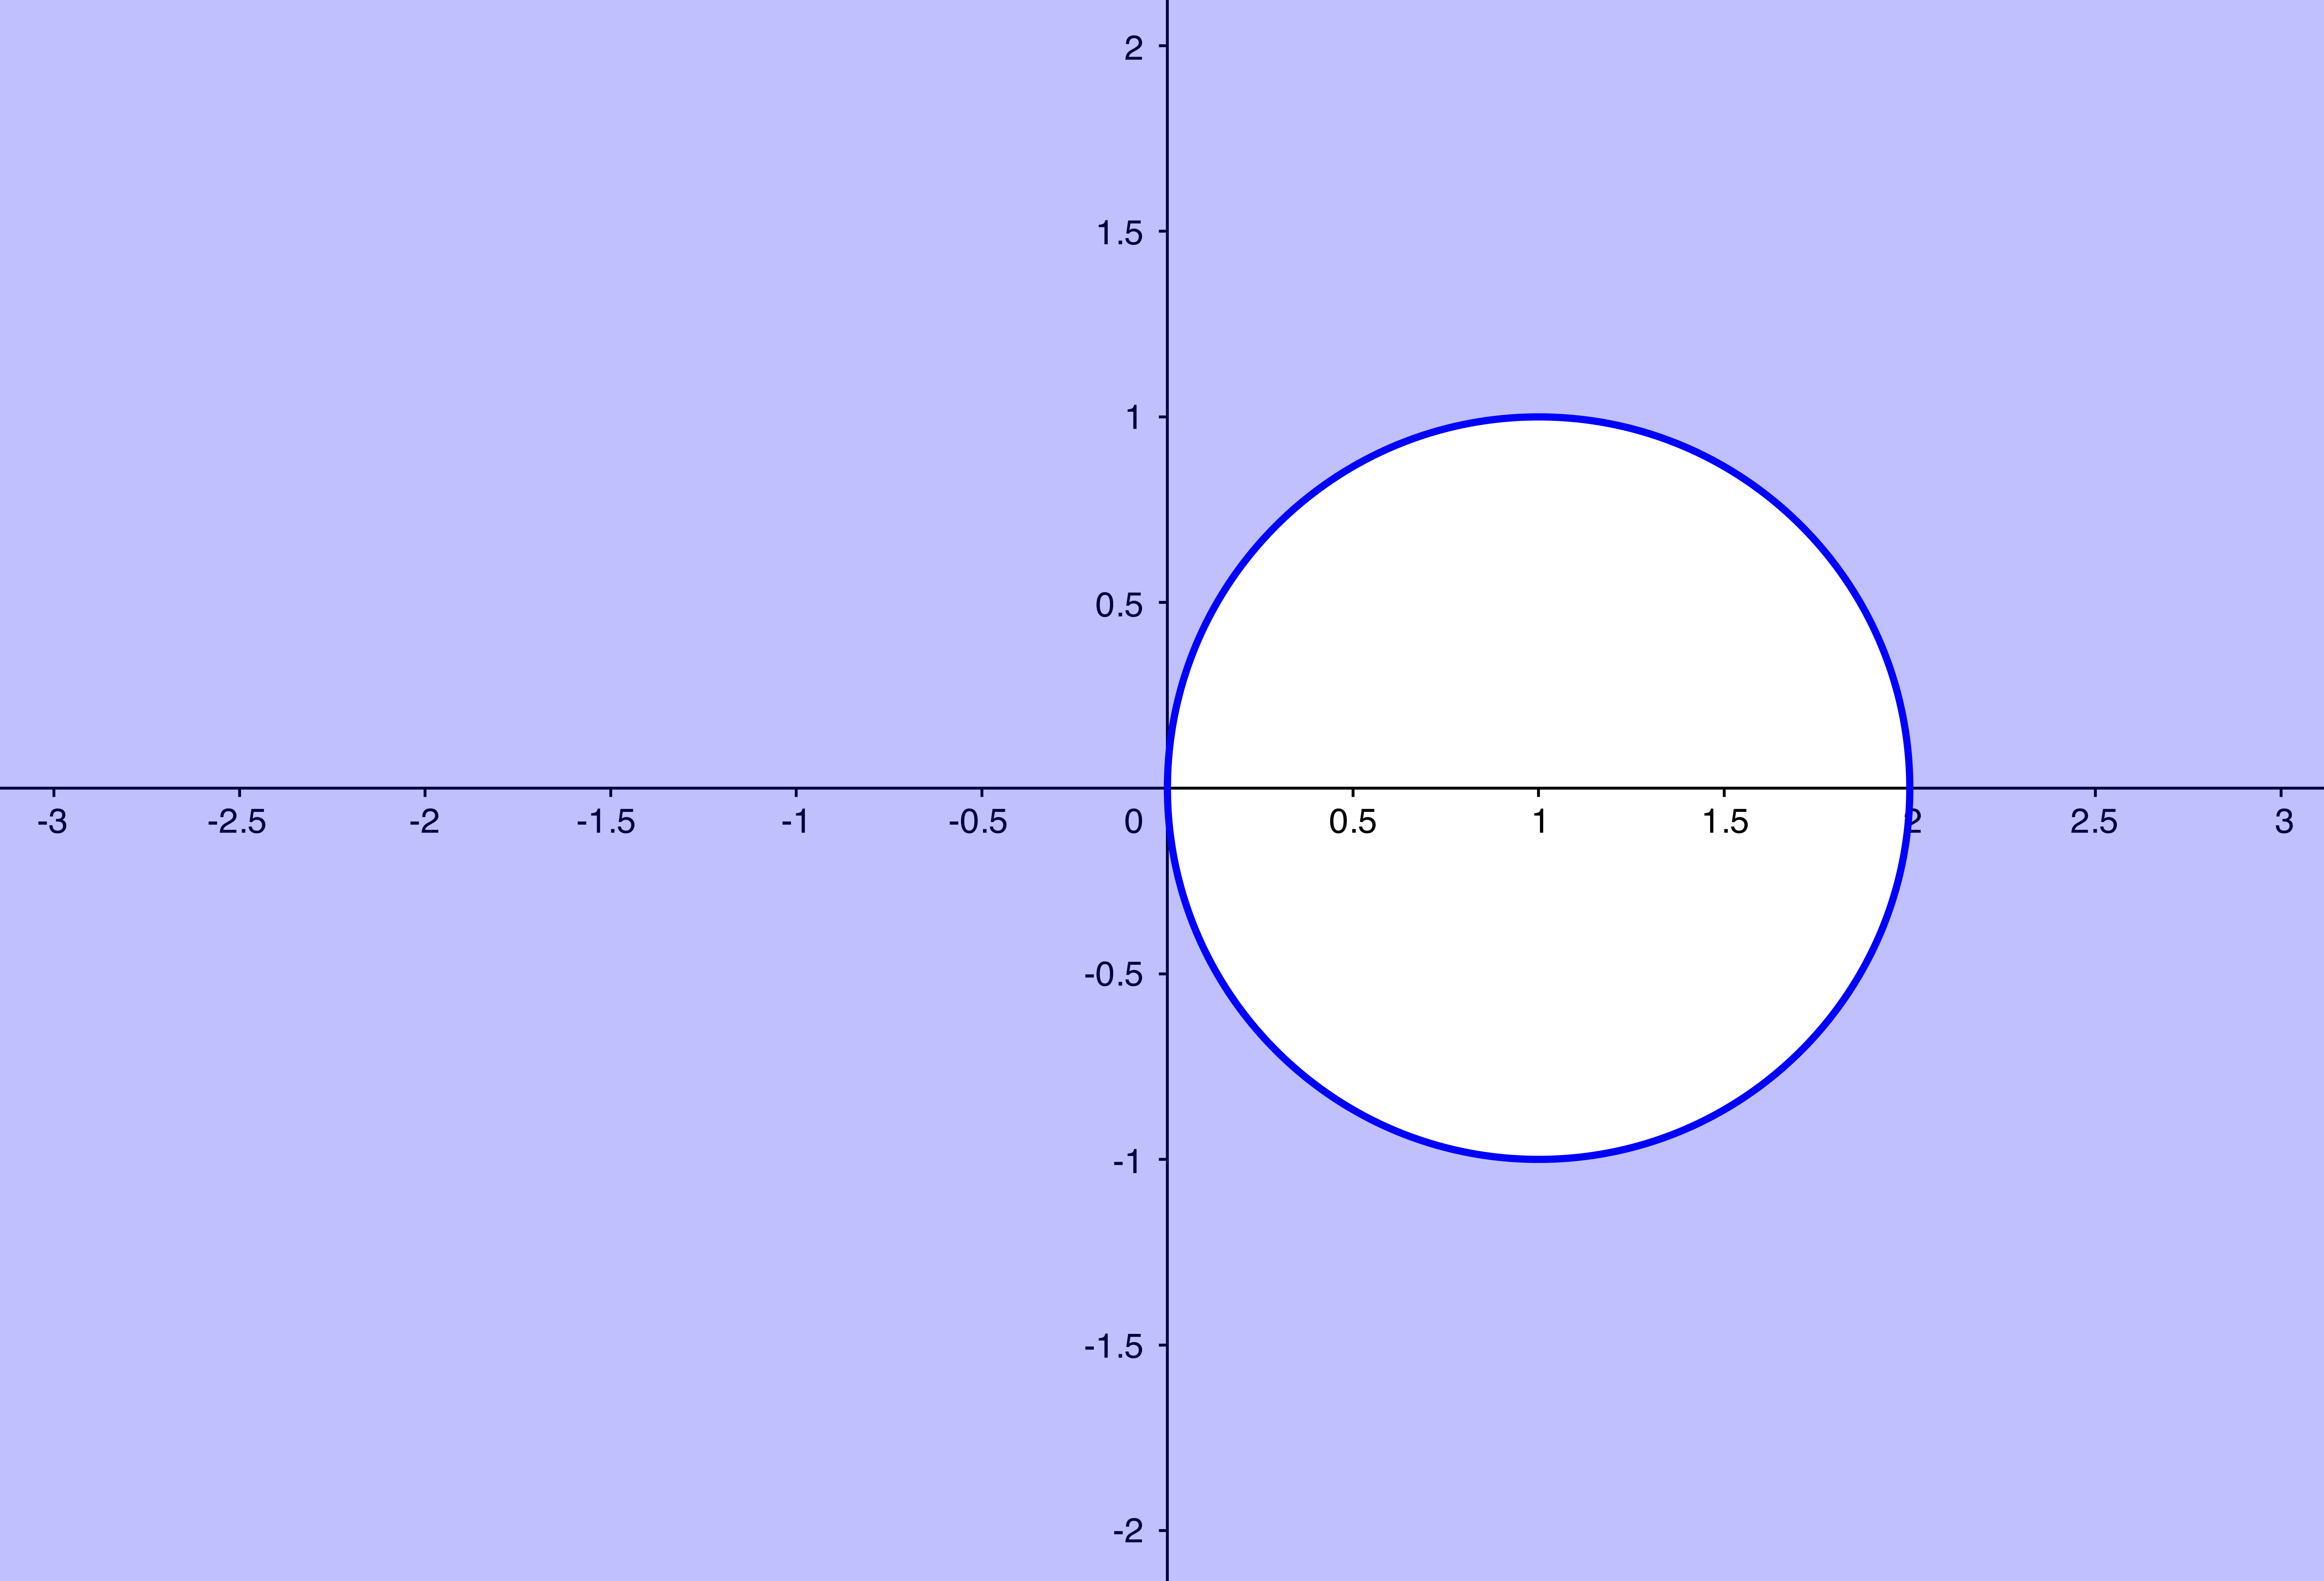
\includegraphics[width=.80\textwidth]{theta5.png}
      \end{center}
     \end{figure}




    \item[\textbf{c.}] Show that the $\theta$-methods are A-stable for $\theta \geq 1/2$. 
    \solution Note that we have already show that for $\theta = 1/2$ the $\theta$-method is A-stable. Let $\theta > 1/2$
    \begin{equation*}
      R(z) = \dfrac{(1 + (1 - \theta)k\lambda)}{ (1 - \theta k\lambda) } = \dfrac{(1 + (1 - \theta)z)}{ (1 - \theta z) }.
    \end{equation*}
    Therefore the stability region is given by 
    \begin{align*}
      \left|\dfrac{(1 + (1 - \theta)z)}{ (1 - \theta z) }\right|&\leq 1\\
      \dfrac{\left|1 + (1 - \theta)z\right|}{\left|1 - \theta z \right|}&\leq 1\\
      \left|1 + (1 - \theta)z\right|&\leq \left|1 - \theta z \right|\\
      \left|1 + (1 - \theta)(x + iy)\right|&\leq \left|1 - \theta(x + iy) \right|\\
      \left|1 + (1 - \theta)x + i(1 - \theta)y\right|&\leq \left|1 - \theta x + i\theta y \right|\\
      (1 + (1 - \theta)x)^2 + (1 - \theta)^2y^2 &\leq (1 - \theta x)^2 + \theta^2 y^2 
    \end{align*}
    Expanding out and collecting like terms, since $\theta > 1/2$ we find that, 
    \begin{align*}
      2x + (1 - 2\theta)x^2 + (1 - 2\theta)y^2 &\leq 0\\
      \dfrac{2}{(1 - 2\theta)}x + x^2 + y^2 &\geq 0\\      
      \left(\dfrac{1}{(1 - 2\theta)}\right)^2 + \dfrac{2}{(1 - 2\theta)}x + x^2 + y^2 &\geq \left(\dfrac{1}{(1 - 2\theta)}\right)^2\\
      \left(x + \dfrac{1}{(1 - 2\theta)}\right)^2 + y^2 &\geq \left(\dfrac{1}{(1 - 2\theta)}\right)^2\\ 
    \end{align*}
    Note that since $\theta > 1/2$ the term $\frac{1}{(1 - 2\theta)} < 0$ and therefore, for some $r > 0$ our stability region looks like, 
    \begin{equation*}
      \left(x  - r\right)^2 + y^2 \geq \left(r\right)^2
    \end{equation*}
    which will always be A-stable. 
  \end{enumerate} 
\end{exercise}
\vspace{.15in}



\begin{exercise}{Problem P31} Consider this Runge-Kutta method, a one-step and implicit interpretation of the multistep midpoint method:
  \begin{align*}
    U^* &= U^n + \frac{k}{2}f(t_n + k/2, U^*)\\
    U^{n + 1} &= U^n + kf(t_n + k/2, U^*)
  \end{align*}
  The first stage is backward Wuler to dertermin an approximation to the value at the midpoint in time. The second stage is a midpoint method 
  using this value. 
  \begin{enumerate}
    \item[\textbf{a.}] Determine the order of accuracy of this method. That is, compute the truncation error accurately enough to know
    the power $p$ in $\tau = O(k^p)$. 
    \solution First we will compute the one-step error $\mathcal{L}^*$ for the first equation. Suppose $U^n = u(t_n)$ and $U^* = u(t_*)$, and 
    not that by substitution we get, 
    \begin{equation*}
      U^* = u(t_n) + \frac{k}{2}f(u(t_*)). 
    \end{equation*}
    Applying the exact solution, and expanding $u(t_n)$ around $t_*$ we get the following, 
    \begin{align*}
      U^* &= \left(u(t_*) - \frac{k}{2}u'(t_*) + O(k^2)\right) + \frac{k}{2}u'(t_*)\\
      U^* &= u(t_*) + O(k^2).
    \end{align*}
    This means that $u(t_*)$ serves as a second order accurate approximation for $U^*$. 
    Proceeding to compute the truncation error, note that we can reorder the second equation 
    and our truncation error for $t^*$ comes from, 
    \begin{equation*}
        \tau^* = \dfrac{u(t_{n + 1}) - u(t_{n})}{k} - f(t_*, U^*)
    \end{equation*}
    Applying our approximation for $U^*$ evaluated at $t^*$ we get $f(t_*, U^*) = f(u(t_*) + O(k^2))$, and substitution of the exact solution
    gives $f(t_*, U^*) = u'(t_*) + O(k^2)$. Expanding $u(t_{n + 1})$ and $u(t_n)$ about $t_*$ we get, 
    \begin{align*}
      \tau^* = \dfrac{1}{k}\biggl( &\left(u(t_*) + \frac{1}{2}ku'(t_*) + \frac{1}{8}k^2u''(t_*) + O(k^3) \right) -\\ 
      &\left(u(t_*) - \frac{1}{2}ku'(t_*) + \frac{1}{8}k^2u''(t_*) + O(k^3) \right)\biggr) - \\
      &(u'(t_*) + O(k^2))
    \end{align*}
    \begin{align*}
      \tau^* &= \dfrac{1}{k}\left(ku'(t_*) + O(k^3)\right) - (u'(t_*) + O(k^2)),\\
       &= O(k^2).
    \end{align*}


    \item[\textbf{b.}] Determine the stability region. Is this method A-stable? Is it L-stable?
    \solution  Applying the test equation $u' = \lambda u$ to our scheme we get the following equations, 
    \begin{equation*}
      U^* = U^n + \frac{1}{2}k\lambda U^*
    \end{equation*}
    \begin{equation*}
      U^{n + 1} = U^n + k\lambda U^*
    \end{equation*}
    Solving for our function $R(z)$ we get the following, 
    \begin{align*}
      U^{n + 1} &= \left(1 + \dfrac{k\lambda}{1 - \frac{1}{2}k\lambda}\right)U^n,\\
      U^{n + 1} &= \left(\dfrac{1 + \frac{1}{2}k\lambda}{1 - \frac{1}{2}k\lambda}\right)U^n,
    \end{align*}
    \begin{equation*}
      R(z) = \dfrac{1 + \frac{1}{2}z}{1 - \frac{1}{2}z}.
    \end{equation*}
    This will result in the same stability region as was plotted for $\theta = 1/2$ of the $\theta$-methods in the previous problem. 
    This method is A-stable. This method is not L-stable, since clearly $\lim_{z \to \infty} |R(z)| \to 1$ and not $0$. 
  \end{enumerate}
\end{exercise}
\vspace{.15in}




\begin{exercise}{Problem P32} Reproduce Table 7.1. In particular, consider the scalar ODE IVP, 
  \begin{equation*}
    u'(t) = \lambda(u(t) - \cos(t))- sin(t), \qquad u(0) = 1
  \end{equation*}
  with the particular value $\lambda = -2100$. Use an implementation of forward Euler, to compute 
  approximations of $u(T)$ for $T = 2$, for the given values of $k$, and report the final-time numerical errors. 
  $|U^n - u(T)|$ as in the Table. Confirm by this experiment that there is a critical value of $k$ around 0.00095 
  where the error finally drops from enormous values to something comparable to, then much smaller than, the solution magnitude itself. 
  \solution Consider the following Matlab code, table71.m which generates the desired table\\

  \textbf{Code:}
  \begin{center}
    \lstinputlisting[basicstyle=\footnotesize]{r1.txt}
  \end{center}
  
  \textbf{Console:}
  \begin{center}
    \lstinputlisting[basicstyle=\small]{r2.txt}
  \end{center}

\end{exercise}
\vspace{.15in}




\begin{exercise}{Problem P33} For a famously stiff problem, consider the heat PDE, 
  \begin{equation*}
    u_t = u_{xx}
  \end{equation*}
  Here $u(t, x)$ is the temperature in a rod of length one $(0 \leq x \leq 1)$ and we set boundary 
  temperatures to zero. For an initial temperature distribution we set one part hotter than the rest:
  \begin{equation}
    u(0, x) = \begin{cases} 1, & 0.25 < x < .5,\\
      0, &\text{otherwise}.
    \end{cases}
  \end{equation}
  Suppose we seek $u(1, x)$, i.e. we set $t_f = 1$. 
  We apply the method of lines(1). That is we discretized the spatial $(x)$
  derivatives using the notation from Chapter 2. Specifically, use $m + 1$ sub-interval, let $h = 1/(m + 1)$
  and let $x_j = jh$ for $j = 0, 1, 2, \dots, m+1$. Now $U_j(t) \approx u(t, x_j).$ By eliminating unknowns $U_0 = 0$
  and $U_{m + 1} = 0$, and keeping the time derivatives as ordinary derivatives we get a linear ODE system of dimensions $m$,
  \begin{equation}
    U(t)' = AU(t)
  \end{equation}
  where $U(t) \in \RR^m$ and $A$ is exactly the matrix in (2.10). For a given $m$, note $U(0)$ is computed from the above formula 
  for $u(0, x)$. 
  
  
  \begin{enumerate}
    \item[\textbf{a.}] Implement both forward and backward Euler on (2). Use backslash for linear solve. 
    \solution

    \textbf{Code:}
    \begin{center}
      \lstinputlisting[basicstyle=\footnotesize]{HEATBEULER.txt}
    \end{center}
    
    \textbf{Code:}
    \begin{center}
      \lstinputlisting[basicstyle=\footnotesize]{HEATFEULER.txt}
    \end{center}



    \item[\textbf{b.}] Now consider the $m = 99$ case, so $h = .01$ and let $k = t_f/N = 1/N$ be 
    the time step length. For BE, compute and show the solution using $N = 100$ time steps. For 
    $FE$, $N = 100$ will generate extraordinary explosion. 

    Determine the largest-possible absolutely stable time step $k$ from the eigenvalues of $A$
    and the the stability region of $FE$. Finally, compare the computation costs of the two runs, 
    by counting floating-point multiplications. You will conclude that an implicit method is indeed effective in this case. 
    \solution Recall that for a linear, constant coefficient, system of IVPs as described by (2), if $A$ is diagonalizable
    then the system can be decoupled in to a system of test equations. 
    \begin{align*}
      U(t)' &= AU(t)\\
      U(t)' &= R \Lambda R^{-1} U(t)\\
      R^{-1}U(t)' &= \Lambda R^{-1}U(t)\\
      (R^{-1}U)(t)' &= \Lambda (R^{-1}U)(t)\\
      W(t)' &= \Lambda W(t)
    \end{align*}
    Let $W(t) = (R^{-1}U)(t)$ and note that $R^{-1}U(t)' = (R^{-1}U)(t)'$ since $R$ is constant. Recall that the eigenvalues of $A$
    are well documented and are given by $\lambda_i = \frac{2}{h} (\cos(i \pi h) - 1)$.
    Applying our test equations to the Forward Euler scheme we get that in order to achieve absolute convergence given spacing $h = .01$,
    \begin{align*}
      |1 + k\lambda_i| &\leq 1\\
      |1 + k\frac{2}{h^2} (\cos(i \pi h) - 1)| &\leq 1\\
      |1 + k\frac{2}{.0001} (\cos(i \pi .01) - 1)| &\leq 1
    \end{align*}
    Note that $\cos(i \pi .01) \approx -1$ and therefore, 
    \begin{align*}
      |1 + k\frac{2}{.0001}(-2)| &\leq 1,\\
      |1 - k\frac{4}{.0001}| &\leq 1,\\
      -1\leq 1 - k\frac{4}{.0001} &\leq 1,\\
      2\geq k\frac{4}{.0001} &\geq 0,\\
      \frac{1}{20000}\geq k &\geq 0.\\
    \end{align*}
    Therefore in order to achieve absolute convergence using forward euler we must take at lease 20,000 times steps. 

    Considering the floating-point multiplications required we find that for each of the 20,000 timesteps we need to 
    perform the $AU(t)$ matrix multiplication, and since $A$ is an $m \times m$ tridiagonal matrix we get a total of $20,000(3m)$ multiplications. 
    However since backward euler is $A$-stable it will produce a quality solution in as little as 100 time steps and
    since it takes only $5m$ multiplications to solve a comparable tridiagonal system, backward euler is substantially better suited for this problem. 
    \newpage
    Here is a script which exports both forward euler and backward euler solutions.\\
    \textbf{Code:}
    \begin{center}
      \lstinputlisting[basicstyle=\footnotesize]{r3.txt}
    \end{center}
    Here is a link to the compiled gifs, \\
    \href{https://github.com/StefanoFochesatto/NumericalDifferentialEquation}{https://github.com/StefanoFochesatto/NumericalDifferentialEquation}

backward 


  \end{enumerate}


\end{exercise}
















\end{document}











 




